%-------------------------------------------------------------------------------
%	PACKAGES EN DOCUMENT CONFIGURATIE
%-------------------------------------------------------------------------------

\documentclass[hidelinks]{uva-inf-article}
\usepackage[english]{babel}

\usepackage{tikz}
\usetikzlibrary{automata,positioning}

\usepackage{listings}

%-------------------------------------------------------------------------------
%	GEGEVENS VOOR IN DE TITEL
%-------------------------------------------------------------------------------

\assignment{Assignment 4}
\assignmenttype{Essay}
\title{Semantic Analysis}

\author{René Kok}
\uvanetid{13671146}

\author{Aram Mutlu}
\uvanetid{13574116}

\docent{Dhr. dr. C.U. Grelck}
\course{Compiler Construction}
\courseid{5062COMP6Y}

\date{\today}

\begin{document}
\maketitle

%-------------------------------------------------------------------------------
%	INTRODUCTIE
%-------------------------------------------------------------------------------

\section{Introduction}
\begin{flushleft}
%-------------------------------------------------------------------------------
%	METHODE
%-------------------------------------------------------------------------------
\newpage
\section{Scoping and symbol tables}
Consider the following CiviC nested function definition:
\begin{lstlisting}[basicstyle=\small, language=C]
int d = 2;

int foo(int a) {
  int b = 1; 
  int c;

  int f(int x) { 
      int b = x + b;
      return b; 
  }

  int g(int x) { 
      c = f( x - b); 
      return c + a;
  }
    
  c = c + g( d - b); 
  return c;
}
\end{lstlisting}
\paragraph{a). What is the value of foo(8), and, more importantly, why?\\}
aaaaa

\newpage
\paragraph{b). Mark every occurrence of a variable identifier in statement position by an arrow to the declaration\\}
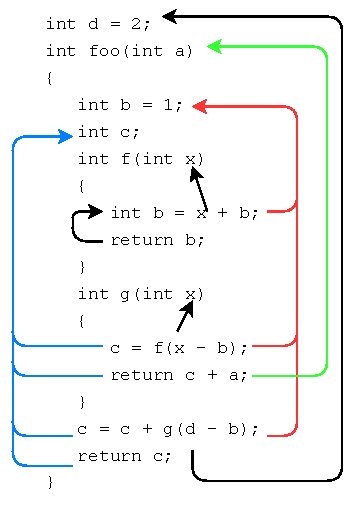
\includegraphics[width=8cm]{images/1b.pdf}
\paragraph{c). Annotate each scope (level) with its symbol table.\\}
baaa
\paragraph{d). Annotate each variable identifier in statement position by a number indicating the relative scope distance to the corresponding declaration.\\}
aaaa
\newpage
\section{Lambda lifting}
\textbf{Manually apply the lambda lifting transformation to the code example of Assignment 4.1.} 
\begin{lstlisting}[basicstyle=\small, language=C]
int d = 2;

int f(int x, int b) {
	int b = x + b;
	return b;
}

int g(int x, int a, int b, int *c) {
	*c = f(x - b);
	return *c + a;
}

int foo(int a, int d) {
	int b = 1;
	int c;

	c = c + g(d - b, *c, b, a);
	return c;
}
\end{lstlisting}
\newpage
\section{Function overloading}
\textbf{Assume we would extend CiviC by function overloading. Describe how 
this extension would affect semantic analysis in the CiviC compiler in general, 
and how you would solve the corresponding problems in detail.\\}
The compiler wouldn't be able to distinguish similarly named functions.
The determination of which function to use for a particular call should 
be resolved at compile time by adding the name of the parameter types to the function name as shown in // TODO: FIGURE.

\end{flushleft}
\end{document}